\section{\twoMode\ $\SOn{2}$-equivariant flow}
\label{s:twoMode}

Our goal is to illustrate and compare continuous symmetry reduction methods
applicable to high-dimensional systems exhibiting chaos.
Dangelmayr,\rf{Dang86} Armbruster, Guckenheimer and Holmes,\rf{AGHO288}
Jones and Proctor,\rf{JoPro87} and Porter and Knobloch\rf{PoKno05} (see
Golubitsky \etal\rf{golubII}, Sect. XX.1) have investigated bifurcations
in 1:2 resonance ODE normal form models to third order in the amplitudes.
We use this model as a starting point from which we derive what may
be the simplest chaotic system with a continuous symmetry. We will
refer to as the {\twomode} system:
\bea
	\dot{z}_1 &=& (\mu_1-\ii\, e_1)\,z_1+a_1\,z_1|z_1|^2
				 +b_1\,z_1|z_2|^2+c_1\,\overline{z}_1\,z_2
	\continue
	\dot{z}_2 &=& (\mu_2-\ii\, e_2)\,{z_2}+a_2\,z_2|z_1|^2
				 +b_2\,z_2|z_2|^2+c_2\,z_1^2 \,,
	\label{eq:DangSO2}
\eea
with $z_1,\,z_2$  complex, and all parameters real valued. This complex
\twomode\ system \refeq{eq:DangSO2} is a 4-dimensional
first order real ODE system,
by substitution $z_1 = x_1 + i\,y_1$, $z_2 = x_2 + i\,y_2$,
\bea
\dot{x}_1 &=& (\mu_1 + a_1 r_1^2 + b_1 r_2^2 + c_1 x_2)x_1 + c_1 y_1 y_2 + e_1 y_1 % double checked DBE 05/22/2014
\continue
\dot{y}_1 &=& (\mu_1 + a_1 r_1^2 + b_1 r_2^2 - c_1 x_2)y_1 + c_1 x_1 y_2 - e_1 x_1 % double checked DBE 05/22/2014
\continue
\dot{x}_2 &=& (\mu_2 + a_2 r_1^2 + b_2 r_2^2)x_2 + c_2 (x_1^2 - y_1^2) + e_2 y_2 % double checked DBE 05/22/2014
\continue
\dot{y}_2 &=& (\mu_2 + a_2 r_1^2 + b_2 r_2^2)y_2 + 2 c_2 x_1 y_1 - e_2 x_2 % double checked DBE 05/22/2014
\continue
		  && \mbox{where } r_1^2 = x_1^2 + y_1^2\, , \quad r_2^2 = x_2^2 + y_2^2
\,.
\label{2mode4D}
\eea
The normal-form analysis leaves us with a large set of parameters
$\left(\mu_1,\mu_2,a_1,a_2,b_1,b_2,c_1,c_2,e_1,e_2\right)$.

Following the time-hallowed tradition of Lorenz\rf{lorenz},
H\'enon\rf{henon} and R\"ossler\rf{ross}, we have played with various
choices of parameters until settling on the set values used in all
numerical \twomode\  calculations presented here:
\beq
	\begin{tabular}{c c c c c c c c c c}
	% after \\: \hline or \cline{col1-col2} \cline{col3-col4} ...
	 $\mu_1$ & $\mu_2$ & $e_1$ & $e_2$ & $a_1$ & $a_2$ & $b_1$ & $b_2$ & $c_1$ & $c_2$ \\
	\hline
	 -2.8	& 1		  & 0	  & 1	  & -1	  & -2.66 & 0	  & 0 	  & -7.75 & 1
	\end{tabular}
	\label{eq:pars}
\eeq
While our choice of parameters is far from the bifurcation values studied
by previous authors \rf{Dang86,AGHO288,JoPro87,PoKno05}, and thus the
model has no physical interpretation, it as the simplest model for the
study of chaotic dynamics in systems with continuous symmetry that we
know of: it is a 4\dmn\ $\SOn{2}$-equivariant model in which the three
dimensional $\SOn{2}$-reduced dynamics are chaotic.

It can be checked by inspection that eqs.~\refeq{eq:DangSO2} are
equivariant under the \Un{1}\ transformation
\beq
(z_1,z_2) \rightarrow   (e^{i {\gSpace}}z_1,e^{i 2{\gSpace}} z_2)
\,.
\ee{Dang86(1.1)aa}
In the real representation \refeq{2mode4D}, the $\SOn{2}$ group action
\refeq{Dang86(1.1)aa} is given by $\ssp'= \exp\left( \theta \Lg\right)\ssp$,
where $\transp{\ssp} =$ \cartpt{x_1, y_1,x_2, y_2}, and $\Lg$ is the Lie algebra
generator
\beq
\Lg  \, =
\left( \begin{array}{cccc}
         0 & -1 & 0 & 0 \\
         1 & 0 & 0 & 0 \\
         0 & 0 & 0 & -2\\
         0 & 0 & 2 & 0
      \end{array} \right)
\,.
\ee{LGTwoMode}
One can easily check that the real \twomode\ system \refeq{2mode4D}
satisfied the equivariance condition \refeq{inftmInv}.

The parameters $\{e_1,e_2\}$ break the $\On{2}$ symmetry of the
Dangelmayr normal form system\rf{Dang86} to an $\SOn{2}$-equivariant
system. As we will show below in \refeq{PKinvEqs1}, only the combination
$(2e_1-e_2)$ matters in the symmetry reduced dynamics, so for simplicity
we set $e_1=0$.

From \refeq{eq:DangSO2} we note that the \eqv\ point \((z_1,z_2)=(0,0)\)
is an invariant subspace, and that $z_1=0$, $z_2 \neq 0$ is a 2\dmn\
flow-invariant subspace,
\beq
  \dot{z}_1 = 0 % Double checked DBE 05/26/2014
\,,\qquad
  \dot{z}_2 = (\mu_2-\ii\, e_2 +b_2 |z_2|^2)\,{z_2} % Double checked DBE 05/26/2014
\,,
\ee{eq:DangSO2spsp}
with a single circular \reqv\ of radius $r_2 = \norm{z_2} = \sqrt{-\mu_2/b_2}$ with
\phaseVel\ $\velRel=-e_2/2$.
    \PC{recheck: is $\velRel=e_2$?} \BB{}{I confirm.} \ES{}{ES: If I write $z_2=e^{i2\phi}z2$, then I get $c=-e_2/2$.}
		\DB{}{I agree with Vagelis... If the phase velocity is defined as written down in Sect. II, s.t. $v(a_q) = c \Lg a_q$, then $v(0,0,x_2,y_2) = (0,0,e_2 y_2, -e_2 x_2)$ and $\Lg (0,0,x_2,y_2) = (0,0,-2 y_2, 2 x_2)$ so $c = -e_2/2$.}
At the origin $\Mvar$ commutes with $\Lg$, and thus can be block-diagonalized
into two $[2\!\times\!2]$ matrices.
% According to {\bf [2012-04-27 Daniel]},
The \cartpt{0,0,0,0} \eqv\ eigenvalues are $\Lyap_1 = \mu_1$ with multiplicity 2 and
$\Lyap_3 = \mu_2 \pm i e_2$. The eigenvectors for $\Lyap_1$ are \cartpt{1,0,0,0} and
\cartpt{0,1,0,0} in the \cartpt{x_1,x_2,y_1,y_2} basis. The eigenvectors for $\Lyap_2$
are \cartpt{0,0,1,0} and \cartpt{0,0,0,1}.

In contrast, $z_2 =0$ is not, in general, a flow-invariant subspace, since the dynamics
\[
  \dot{z}_1 = (\mu_1-\ii\, e_1)\,z_1+a_1\,z_1|z_1|^2
\,,\qquad
  \dot{z}_2 = c_2\,z_1^2
\,.
\]
take the flow out of the $z_2 =0$ plane.
    \PC{should we check if anything of interest happens for $c_2 = 0$? }


\subsection{Invariant polynomial bases}
\label{s:invPol}

Consider the \statesp\ of a dynamical system
constructed from two complex Fourier modes\rf{Dang86,AGHO288,PoKno05}
$m=(1,2)$, with the $\SOn{2} \simeq \Un{1}$ group action given by
rotation \refeq{Dang86(1.1)aa}. In this
case it is easy to construct a set of four real-valued
$\SOn{2}$ invariant polynomials
\bea
u &=& {z}_1 \overline{z}_1
    \,,\quad
v = {z}_2 \overline{z}_2
    \continue
w &=& z_1^2 \overline{z}_2 + \overline{z}_1^2 {z}_2
    \,,\quad
q = (z_1^2 \overline{z}_2 - \overline{z}_1^2 {z}_2)/\ii
\,.
\label{Dang86(1.2)PK}
\eea
The polynomials $\{u,v,w,q\}$ are
linearly independent, but related through one syzygy,
\beq
w^2+q^2 - 4\,u^2v = 0 % Double checked syzygy is satisfied by eq Dang86(1.2)PK DBE 05/22/2014
  \,,
\label{eq:syzPK}
\eeq
which confines the dynamics to a 3-dim\-ens\-ion\-al $\pSRed=\pS/\SOn{2}$
\reducedsp\ manifold, a symmetry-invariant repre\-sent\-ati\-on of the
4-dim\-ens\-ion\-al \SOn{2} equivariant dynamics. By construction $u \geq
0$, $v \geq 0$, but $w$ and $q$ can be of either sign. That is explicit
in in polar coordinates $ {z}_1 = |u|^{1/2} e^{\ii\phi_1}$, $ {z}_2 =
|v|^{1/2} e^{\ii\phi_2}$, where the  $w, q$ invariants take the form
\bea
w &=& 2\,\Re(z_1^2 \overline{z}_2) = 2\,u |v|^{1/2} \cos \psi %Triple checked DBE 05/22/2014
\continue
q &=& 2\,\Im(z_1^2 \overline{z}_2) = 2\,u |v|^{1/2} \sin \psi %Triple checked DBE 05/22/2014
\,,
\label{Dang86(1.2)polar}
\eea
where $\psi = 2 \phi_1 - \phi_2$.

The dynamical equations for \invpt{u,v,w,q} follow from the chain rule
\( %beq
 \dot{ u}_i= \sum_j ({\partial u_i}/{\partial \ssp_j}) \, \dot{\ssp}_j
 \,
\) %ee{HilbChainRl}
. This yields
\bea
  \dot{u} &=& \overline{z}_1 \dot{z}_1 + {z}_1 \dot{\overline{z}}_1 % Triple checked DBE 05/22/2014
\,,\qquad
  \dot{v} = \overline{z}_2 \dot{z}_2 + {z}_2 \dot{\overline{z}}_2 % Triple checked DBE 05/22/2014
\continue
  \dot{w} &=& 2 \,\overline{z}_2 {z}_1 \dot{z}_1 % Triple checked DBE 05/22/2014
           + 2\,{z}_2 \overline{z}_1 \dot{\overline{z}}_1
           + {z}_1^2 \dot{\overline{z}}_2
           + \overline{z}_1^2 \dot{z}_2
\continue
  \dot{q} &=&  (2\,\overline{z}_2 {z}_1 \dot{z}_1 % Triple checked DBE 05/22/2014
           - 2\,{z}_2 \overline{z}_1 \dot{\overline{z}}_1
           + {z}_1^2 \dot{\overline{z}}_2
           - \overline{z}_1^2 \dot{z}_2
           )/\ii
\label{PKinvEqs}
\eea
Substituting  \refeq{eq:DangSO2} into \refeq{PKinvEqs} we obtain the set
of 4 $\SOn{2}$-invariant equations,

\bea
  \dot{u} &=& 2\,\mu_1\,u+2\,a_1\,u^2+2\,b_1\,u\,v+c_1\,w % Triple checked DBE 05/22/2014
\continue
  \dot{v} &=& 2\,\mu_2\,v+2\,a_2\,u\,v+2\,b_2\,v^2+c_2\,w % Triple checked DBE 05/22/2014
\continue
  \dot{w} &=& (2\,\mu_1+\mu_2)\,w+(2a_1+a_2)\,u\,w+(2b_1+b_2)\,v\,w % Triple checked DBE 05/22/2014
\ceq
             +\, 4c_1\,u\,v + 2c_2\,u^2 +(2e_1 - e_2)\,q
\label{PKinvEqs1}\\
  \dot{q} &=& (2\mu_1+\mu_2)\,q+(2a_1+a_2)\,u\,q
\ceq
             +(2b_1+b_2)\,v\,q
             -(2e_1-e_2)\,w % Triple checked DBE 05/22/2014
\,.
\nnu
\eea
Note that the $\On{2}$-symmetry breaking parameters
 $\{e_1,e_2\}$ of the
Dangelmayr normal form system\rf{Dang86} appear only in the
relative phase combination $(2e_1-e_2)$.
%[2012-07-31 Evangelos]
Using the syzygy \refeq{eq:syzPK} we can
eliminate $q$ from \refeq{PKinvEqs1} to get
    \PC{
    Note that $4u^2v-w^2 = 4u^2v(1-\cos^2\psi)$, so
    no serious singularity is introduced this way. Perhaps
    write equations of $(u,v,\cos \psi)$ as in the
    ChaosBook exercises?
    }
\bea
  \dot{u} &=& 2\,\mu_1\,u+2\,a_1\,u^2+2\,b_1\,u\,v+c_1\,w \nonumber % Triple checked DBE 05/22/2014
\\
  \dot{v} &=& 2\,\mu_2\,v+2\,a_2\,u\,v+2\,b_2\,v^2+c_2\,w \label{PKinvEqs1syz}  % Triple checked DBE 05/22/2014
\\
  \dot{w} &=& (2\,\mu_1+\mu_2)\,w+(2a_1+a_2)\,u\,w+(2b_1+b_2)\,v\,w % Triple checked DBE 05/22/2014
\ceq
             +\, 4c_1\,u\,v + 2c_2\,u^2 +(2e_1 - e_2)(4u^2v-w^2)^{1/2}\,
  \nonumber
\eea

One can now either investigate the dynamics in this invariant basis or
plot the `image'\rf{GL-Gil07b} of solutions computed in the equivariant
basis \refeq{eq:DangSO2} in terms of invariant polynomials
\refeq{Dang86(1.2)PK}.

%\item[2012-04-29 Predrag]
For the 4\dmn\ model at hand we find the invariant polynomials \refeq{PKinvEqs1}
and the polar coordinates \refeq{Dang86(1.2)polar} very useful for cross-checking the
full \statesp\ $\transp{\ssp} =$ \cartpt{x_1, x_2,y_1, y_2} calculations.
But even
for the simplest conceivable $\SOn{2}$ 4-dimensional flow their
construction requires a bit of algebra, and we do not know
how to carry out such constructions for very high\dmn\ flows,
such as the \KS\ flow, and the Navier-Stokes flow.


\subsubsection{\Eqva\ of the symmetry-reduced dynamics}
\label{s:eqva}

The first step in elucidating the geometry of attracting
sets is the determination of their \eqva. We shall now show that the problem of determining
the \eqva\ of the symmetry-reduced \twomode\ \refeq{PKinvEqs1} system \invpt{u*,v*,w*,q*} can be reduced to finding the roots of a multinomial expression.\ES{2014-05-15}{Why do you count complex
solutions as equilibria?}
%[2012-04-28 Predrag]
First, let we define
\beq
A_1= \mu_1+a_1\,u+b_1\,v
    \,,\qquad
A_2 = \mu_2+a_2\,u+b_2\,v
\ee{PKinvEqs2a}
then rewrite \refeq{PKinvEqs1} as
%     \newpage
\bea
  0  &=&  2\,A_1\,u +c_1\,w % Double checked DBE 05/24/2014
    \,,\qquad
  0  =  2\,A_2\,v +c_2\,w % Double checked DBE 05/24/2014
\continue
  0  &=& (2\,A_1+ A_2)\,w
          +2\,\left(c_2\,u+2\,c_1\,v\right)\,u % Double checked DBE 05/24/2014
          \ceq
		  + (2e_1-e_2)\,q
\label{PKinvEqs3}\\
  0  &=& (2\,A_1+ A_2)\,q - (2e_1-e_2)\,\,w % Double checked DBE 05/24/2014
\nnu
\eea
We already know \invpt{0,0,0,0} and \invpt{0,-\mu_2/b_2,0,0} roots, so we are looking only
for the $u>0$, $v>0$, $w,q \in \reals$ solutions; there could be problems\ES{2014-05-15}{What problems?}
from the non-generic roots with either $w=0$ or $q=0$, but not both
simultaneously, syzygy \refeq{eq:syzPK} precludes that. $w$ and/or $q$
can be eliminated by obtaining the following relations from \refeq{PKinvEqs3}:
\bea
	w  &=& - \frac{2\,u}{c_1}\,A_1 = - \frac{2\,v}{c_2}\,A_2 % Double checked DBE 05/24/2014
	\continue
	q &=& \frac{2(-2e_1+\,e_2)\,u\,v}{c_2\,u+2\,c_1\,v} . % Having issues with this DBE 05/24/2014... potentially drops a w = 0 root.
	\label{PKinvEqs4}
\eea
Substituting \refeq{PKinvEqs4}\DB{}{I think getting to the equation for $q$ throws out a potential $w = 0$ root. Do the first two equations then imply that u,v = 0? If, so then q = 0 and there's no problem, but I don't think that's the most general case.} into \refeq{PKinvEqs3} we get two bivariate
polynomials roots of which are the \eqva\ of the system \refeq{PKinvEqs1}:
\bea
	f(u,v) &=& c_2\,u\,A_1 - c_1\,v\,A_2 = 0 \,,\qquad  \nonumber
	\\
	g(u,v) &=&
 \left(4\,A_1^2 u^2 - 4\,c_1^2\,u^2 v\right)\left(c_2\,u+2\,c_1\,v\right)^2 \label{PKinvEqs5} %Double checked DB 04-30-2012
	\ceq
	+\,4\,c_1^2\,(-2e_1+e_2)^2\,u^2\,v^2 = 0
\,,
	\\
	deg(f) &=& 2, \, deg(g) = 6 \nonumber
\,.
\eea
%\DBedit{DB: Not sure where this factor of 2 comes from in $w =
%-\frac{2}{e_2} (2\,A_1+ A_2)\,q $. From the last equation in
%\refeq{PKinvEqs3}, I get $w = -\frac{1}{e_2} (2\,A_1+ A_2)\,q$.
%Therefore, I get I get  $q = \frac{2 e_2\,u\,v}{c_2\,u+2\,c_1\,v}$}
%2012-04-29 Predrag: thanks!

% \DBedit{DB: I get $g(u,v) = \left(w^2 - 4\,u^2
% v\right)\left(c_2\,u+2\,c_1\,v\right)^2 +\,4\,e_2^2\,u^2\,v^2 = 0$}
%2012-04-29 Predrag: thanks!
%2012-04-29 Predrag: should have I used the syzygy \refeq{eq:syzPK},
%$w^2 - 4\,u^2v = -q^2$ DB: If you plug the syzygy in you trivially get zero....

We divide the common multiplier $u^2$ from the second equation and by doing
so, eliminate one of the two roots at the origin, as well as
and the \cartpt{0,-\mu_2/b_2,0,0} root. Furthermore,
we scale the parameters and variables as
$\tilde{u} = c_2\,u$,
$\tilde{v} = c_1\,v$,
$\tilde{a_1} = a_1/c_2$,
$\tilde{b_1} = b_1/c_1$,
$\tilde{a_2} = a_2/c_2$,
$\tilde{b_2} = b_2/c_1$,
to finally get
\bea
\tilde{f}(\tilde{u},\tilde{v}) &=&
  \tilde{u}\,\tilde{A}_1 - \tilde{v}\,\tilde{A}_2 = 0 %Double checked DB 04-30-2012
\,,\qquad deg(f) = 2 \label{PKinvEqs5a}
\\
\tilde{g}(\tilde{u},\tilde{v}) &=&  %Double checked DB 04-30-2012
 \left(\tilde{A}_1^2
 - c_1\,\tilde{v}\right)
 \left(\tilde{u}+2\,\tilde{v}\right)^2
 +e_2^2\,\tilde{v}^2 = 0
\,,
\ceq
   deg(g) = 4 \label{PKinvEqs5b}
\\
 && \mbox{where }
\tilde{A}_1 = \mu_1+\tilde{a_1}\,\tilde{u}+\tilde{b_1}\,\tilde{v}
\,,\ceq
\qquad\quad \tilde{A}_2 = \mu_2+\tilde{a_2}\,\tilde{u}+\tilde{b_2}\,\tilde{v}
\,,
\label{PKinvEqs5c}
\eea

In order to find \reqva\ of the \twomode\ system, one has to solve two bivariate
polynomials \refeq{PKinvEqs5a} which, in general, is not a trivial task. However,
for the choice of parameters given by \refeq{eq:pars}, \refeq{PKinvEqs5a} yields
$\tilde{v} = (\mu_1 + \tilde{a}_1 \tilde{u})/(\mu_2 + \tilde{a}_2
\tilde{u})$. By substituting this into \refeq{PKinvEqs5b},
we can solve this equation which becomes a fourth order polynomial in $u$. Only
non-negative, real roots of this polynomial has a correspondence in the \twoMode\
\statesp\ since $u$ and $v$ are the squares of first and second mode amplitudes 
respectively. Two roots satisfy this condition, the \eqv\ at the origin:
\beq
	\invpol_{\EQV{}} = (0,0,0,0)^T , %\qquad \mbox{(double)}
\ee{eq:origin}
and the \reqv :
\beq
	\invpol_{\REQV{}{}} = (0.193569,0.154131,-0.149539,-0.027178)^T\,.
\ee{eq:reqv}
Note that by setting $b_2 = 0$, we send the \reqv\ at $\invpol =
(0,-\mu_2/b_2,0,0)$ to infinity. Thus, \refeq{eq:reqv} is the only \reqv\ 
of the \twomode\ system for our particular choice of parameters in \refeq{eq:pars}. 
This \reqv\ traces out its group orbit in the \SOn{2}-equivariant, real-valued
\statesp . One representative point on this orbit can be chosen as:
\[
  \left(x_1, y_1, x_2, y_2\right) = \left(0.439966, 0, -0.386267, 0.070204\right) .
\]


%\subsection{No chaos when the reflection symmetry is restored}
%\label{s:dfsafs}

%Before finishing our discussion of invariant polynomials, we have to make an
%important observation: Consider the case when the reflection symmetry breaking
%parameters $e_{1,2}$ in \refeq{eq:DangSO2} set to $0$. This restores 
%$\sspC_{1,2} \rightarrow \bar{\sspC}_{1,2}$ symmetry, which is broken in 
%the \SOn{2}-equivariant case. Now, note that setting $ e_{1,2} $ to $0$ 
%decouples $q$ in \refeq{PKinvEqs1} from the rest of the invariant polynomials.
%Furthermore, time derivative of $q$ becomes linear in itself, which can be
%expressed as:
%\beq
    %\dot{q} = \xi (u, v) q \, , 
%\ee{e-qlinearq}
%where $\xi$ is not a function of $q$. Hence we can write
%the time evolution of $q$ as
%\beq
    %q(t) =  e^{\int_0^t d \tau \xi (u(\tau), v(\tau))} q(0) \, . 
%\ee{e-qO2solq} 
%If we assume that the flow is bounded, then we can also assume that a long time 
%average of $\xi$ exists. Sign of this average would determine the long term 
%behavior of $q(t)$; it will either diverge or vanish depending on the sign of 
%$\langle \xi \rangle$ being positive or negative respectively. In either case, we 
%are left with three invariant polynomials that are related to each other by the 
%syzygy \refeq{eq:syzPK}, thus the flow is effectively confined on a two dimensional
%manifold, hence cannot exhibit chaos. We must stress that this is a special result
%when one has only first and second Fourier mode, and the equivariant normal form 
%includes terms upto the third order. 

\subsection{Visualizing \twomode\ dynamics}
\label{s:visual}

\begin{figure}%[H]
\centering
(a)\!\!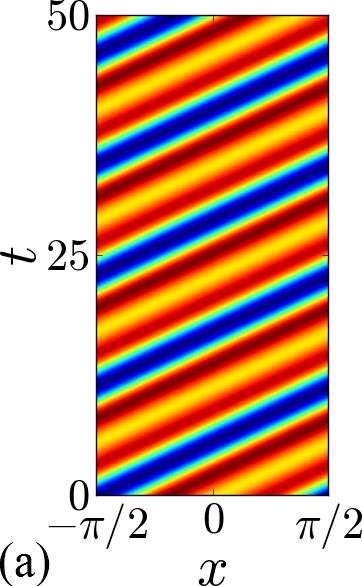
\includegraphics[width=0.22\textwidth]{2modes-conf-reqv}%
(b)\!\!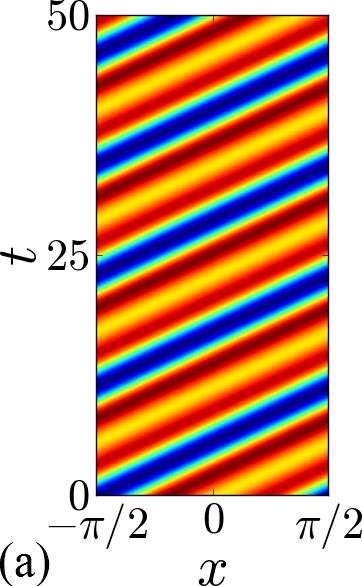
\includegraphics[width=0.22\textwidth]{2modes-conf-reqv}%
\caption{(Color online)
The \reqv\ \REQV{}{} in
 (a) the full \statesp, becomes an \eqv\ in
 (b) the symmetry-reduced configuration space.
}
\label{fig:2modes-conf-reqv}
\end{figure}

\begin{figure}%[H]
\centering
(a)\!\!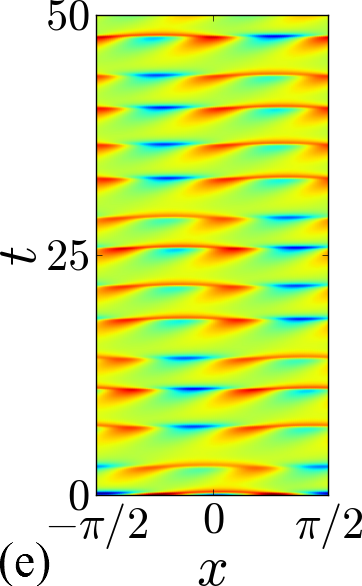
\includegraphics[width=0.22\textwidth]{2modes-conf-ergodic}
(b)\!\!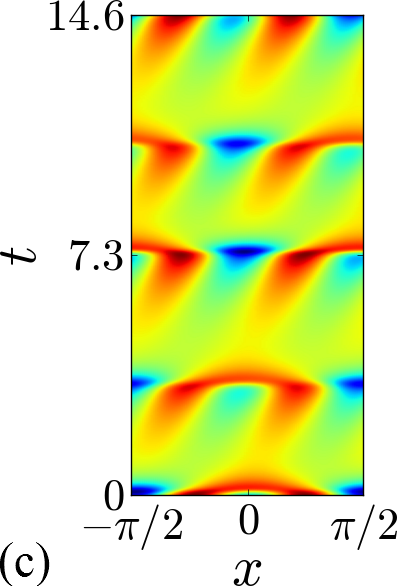
\includegraphics[width=0.22\textwidth]{2modes-conf-rpo}%
\caption{(Color online)
 (a) A typical ergodic trajectory of the \twomode\ system in the
 symmetry-reduced configuration space; clearly the unstable \reqv\
 \REQV{}{} in \reffig{fig:2modes-conf-reqv}\,(b) is far from a typical
 state.
 (b) Two repeats of \rpo\ \cycle{01}  (note the different time scale),
 in the symmetry-reduced configuration space. The dynamics is mostly
 dominated by the $m=1$ Fourier mode, interspersed by rapid shifts by
 $\approx \pm L/2$, dominated by the  $m=2$ Fourier mode.
}
\label{fig:2modes-conf}
\end{figure}

\begin{figure}%[H]
\centering
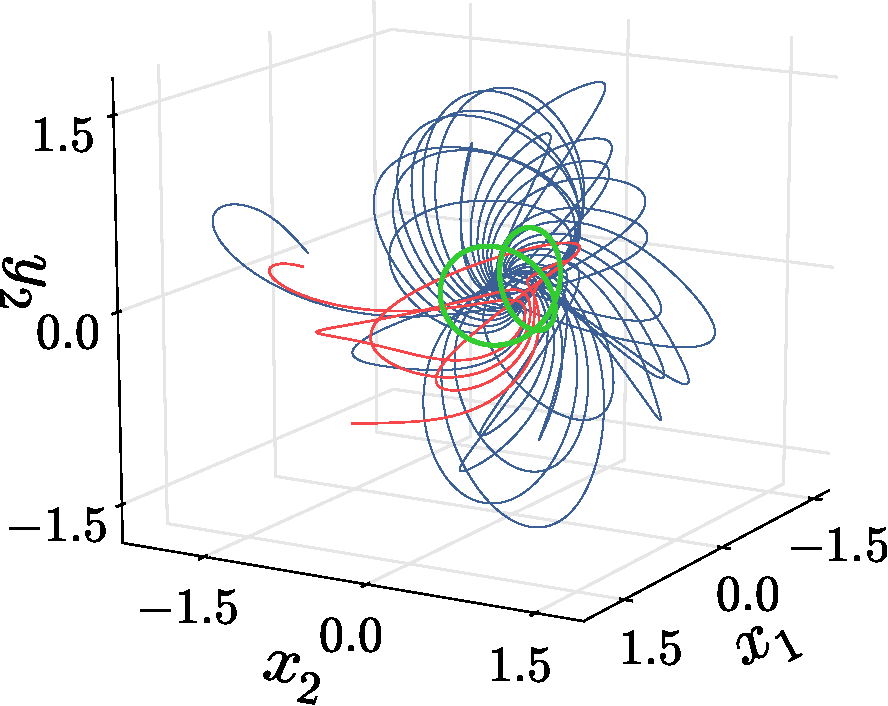
\includegraphics[width=0.45\textwidth]{2modes-ssp}
\caption{(Color online)
The same trajectories as in \reffig{fig:2modes-conf},
colored green, red and blue respectively,
in a 3D projection of the 4\dmn\ \statesp.
}
\label{fig:2modes-ssp}
\end{figure}

\begin{figure}%[H]
\centering
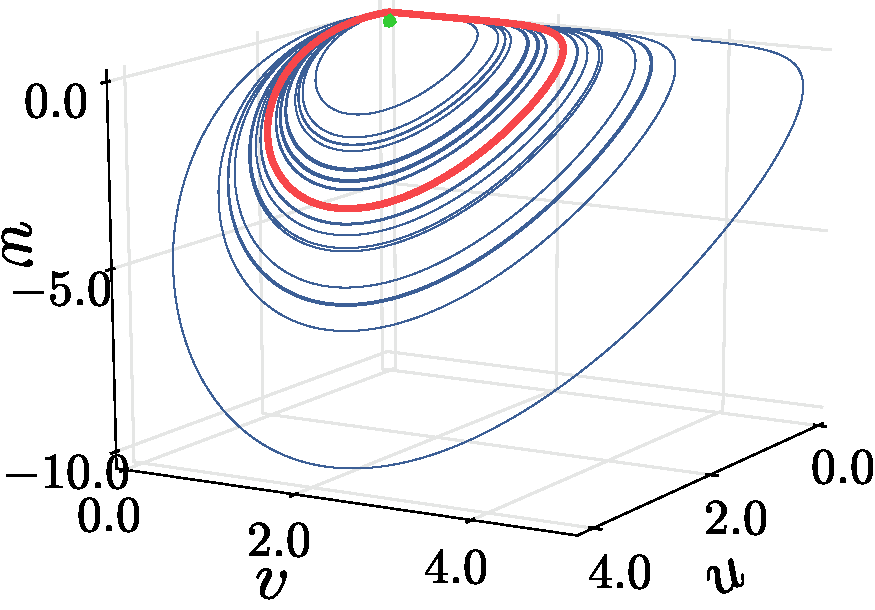
\includegraphics[width=0.45\textwidth]{2modes-invpol}
\caption{(Color online)
The same trajectories as in \reffig{fig:2modes-conf} and
\reffig{fig:2modes-conf-reqv}\,(a), colored green, red
and blue respectively, in a terms of 3 invariant polynomials.
The \reqv\ \REQV{}{} is now reduced to an \eqv, the green point.
}
\label{fig:2modes-invpol}
\end{figure}

\begin{figure}%[H]
\centering
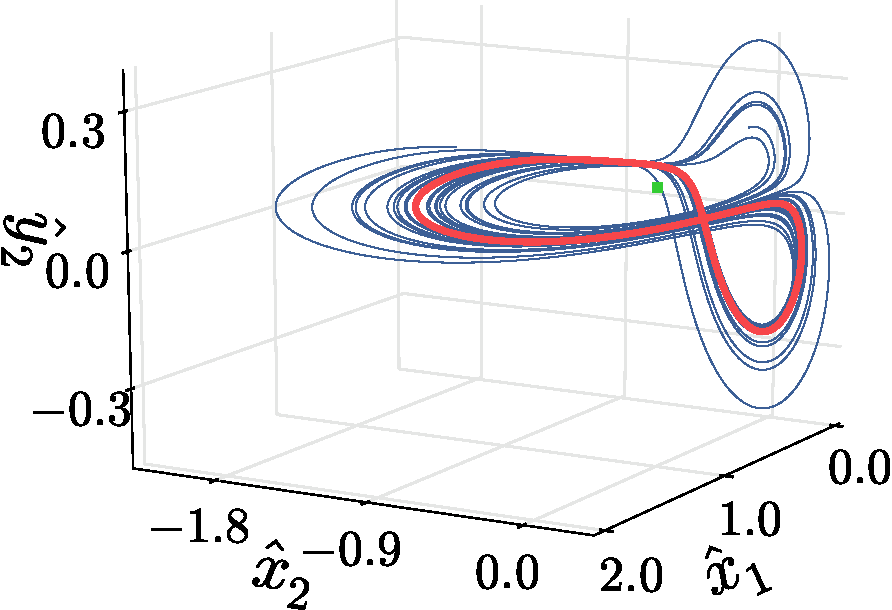
\includegraphics[width=0.45\textwidth]{2modes-sspRed}
\caption{(Color online)
The same trajectories as in \reffig{fig:2modes-conf} and
\reffig{fig:2modes-conf-reqv}\,(a), colored green, red
and blue respectively, in the 3\dmn\  first Fourier mode \slicePlane. The
\reqv\ \REQV{}{} is now reduced to an \eqv, the green point. In contrast
to the invariant polynomial representation \reffig{fig:2modes-invpol},
the qualitative difference between shifts by $\approx L/2$ and $\approx
-L/2$ in near passages to the {\sliceBord} is very clear, and it leads to
the unimodal Poincar\'e return map of \reffig{fig:psectandretmap}.
}
\label{2modes-sspRed}
\end{figure}

\PC{2014-07-14
Why $\pm L/2$ in \reffig{fig:2modes-conf} and
\reffig{fig:2modes-conf-reqv} and not $\pm \pi$?
}
\ES{2014-05-15}{I have replaced the second-mode slice, double-angled
figure in \reffig{2modes-conf-reqv}\,(b) with one resulting by integrating on the
$(0,0,1,0)$ slice, for consistency with panel (c). I hope Burak will
replace it with a publication quality figure of the same representation.
The trick of angle doubling will be introduced in its own section. }

We visualize the dynamics of the \twomode\ system in four different
representations: 3D projections of the four-dimensional real valued
\statesp\ and invariant polynomials, in the 3D \slicePlane\ and on the 2D
configuration space plots on which the color-coded field $u(\conf,\zeit)$
is defined as follows:
\bea
	u(\conf, \tau) &=& \sum_{k=-2}^{2} \sspC_k(\zeit) e^{i k \conf}\, ,
	\continue && \mbox{where} \, \sspC_{-k} = \sspC_k^* \, \mbox{and} \,
	\sspC_0 = 0
\, .
\eea
\refFig{fig:2modes-conf}, \reffig{fig:2modes-conf-reqv}\,(a)
and \reffig{2modes-sspRed} show the sole \reqv\
\REQV{}{}, the \rpo\ \cycle{01}, and an ergodic trajectory of the
\twomode\ system in the four different representations discussed above.
Note that translation of the \reqv\ in the configuration space
\reffig{fig:2modes-conf-reqv}\,(a), corresponds to the \SOn{2} rotations in
the \statesp\ of Fourier modes in \reffig{2modes-ssp} (green curve) and
these orbits correspond to a single point in the symmetry reduced
representations of \reffig{fig:2modes-invpol} and \reffig{2modes-sspRed}.
Note also that the \rpo\ \cycle{01} translates/rotates as it advances in
configuration space (\reffig{fig:2modes-conf}\,(b)) and in the
equivariant \statesp\ \reffig{2modes-sspRed} (\reffig{2modes-ssp}),
whereas in the symmetry reduced plots (\reffig{fig:2modes-invpol} and
\reffig{2modes-sspRed}), it closes onto itself after one period.
